\chapter{Experiments}\label{experiments}
In this section, I present experiments on text classification on collected datasets. The main \textbf{target} dataset for evaluations is the BABE dataset due to its high quality and properties.

Because of novelty of the CWNC I also perform a baseline evaluation on this dataset, but furthermore it is not tuned anymore, nor evaluated.
I follow the current standard approaches and use pre-trained transformers for further pre-training and fine-tuning. 

A brief summary of the models tested can be found in the following:




\subsection{Czech monolingual models}
\begin{itemize}
    \item \textbf{RobeCzech} \cite{strakarobeczech} - RoBERTa-based model with 125M parameters. Like its original counterpart, it is trained with the \gls{mlm} task, on 4,917M tokens of Czech corpora.
    \item \textbf{Czert} \cite{sido-etal-2021-czert} - BERT-based model with 110M parameters, trained with \gls{nsp} tasks. All Together trained on 37GB of text. 
    \item \textbf{FERNET-C5} \cite{lehevcka2021comparison} - BERT-based model trained with the \gls{mlm} and \gls{nsp} task on 93GB of text from the Common Crawl project.
    \item \textbf{FERNET-News} \cite{lehevcka2021comparison} - RoBERTa-based model trained with \gls{mlm} task on 20GB of Czech News text.
\end{itemize}






\subsection{Multi-lingual models}
\begin{itemize}
    \item \textbf{SlavicBert} \cite{arkhipov2019tuning} - BERT-based model with 179M parameters, trained on four languages: Russian, Bulgarian, Czech, and Polish. The model is trained on all 4 languages at once. The model is not trained from scratch, but it is a fine-tuned version of mBERT.
    \item \textbf{mBERT} - BERT-based model with 179M parameters trained on corpora of 104 languages, including Czech, with MLM task.
\end{itemize}




\section{Experimental setup}
All models are fetched, trained, and evaluated using the HuggingFace API. The maximum sequence length is set to 128 tokens. All the parameters can be seen in the Appendix.
Everything is evaluated using 10-fold cross-validation. The evaluation metric for all experiments is the F1 score with macro averaging\footnote{The score is averaged over all (2) classes.}. 

A small portion (15\%) of the target dataset is left aside as a \textbf{test set} at the beginning and used only for the final evaluation to ensure that no test data leak into the training data.

All training has been done on the RCI cluster node with 4 x NVIDIA Tesla V100 with 32GB GPU graphic memory.





 \section{Baseline setup}
 As a baseline, all Czech models are fine-tuned on BABE and evaluated using a 10-fold stratified cross-validation. The hyperparameters used are the same as those used by the authors of the BABE \cite{Spinde2021MBIC}. However, the authors used early stopping together with cross-validation and used the validation split inside CV to early stop, which allows the model to "see" the test during the tuning before the evaluation. 
 
 Using early stopping would require another split for validation, but at this point, the size of the training data is already shrunk significantly. Hence, I did not use early stopping with CV at all and fixed the number of epochs to 3 as suggested by the authors of BERT \cite{devlin2019bert} . 
 All other hyperaparemeters remained unchanged. AdamW optimizer is used with an initial learning rate of 5e-5 and a batch size of 64.
 
 The baseline evaluation of all Czech models used can be seen in table \ref{table:3}. The final F1 score is averaged across all folds. For further tuning, the best model, \textbf{FERNET-C5}, is chosen.
 

 
 \begin{table}
\makebox[\textwidth][c]{
\begin{ctucolortab}
\begin{tabular}{c||c|c|c|c|c|c}
 \textbf{target}\textbackslash \textbf{models} & \textbf{Czert} & \textbf{RobeCzech} & \textbf{mBERT} & \textbf{FERNET-C5} & \textbf{FERNET-News} & \textbf{SlavicBERT}\\
 \hline
 \hline
 \textbf{BABE} & 0.739 & 0.773 & 0.743 & \textbf{0.78} & 0.644 & 0.762 \\
 \hline
 \textbf{CWNC} & 0.726 & \textbf{0.758} & 0.734 & 0.689 & 0.602 & 0.729 \\
\end{tabular}
\end{ctucolortab}
\caption{F1 scores of baseline fine-tuning. Best scores for each dataset are highlighted.}
\label{table:3}
}
\end{table}

 
 
 
 
\newpage

 \section{Hyperparameter tuning}
I restricted the search space only to the combinations of:
 \begin{itemize}
     \item \textbf{Batch size} $\in \{16,32\}$
     \item \textbf{Learning rate} $\in $ \{2e-5,3e-5,5e-5\}
     \item \textbf{Epochs} $\in \{2,3,4\}$
 \end{itemize}
 
 As the authors of the original BERT paper suggest.  After running the grid search, the overall best parameters were:
 \begin{center}
      \{learning\_rate = 3e-5,batch\_size = 32, epochs=3\}
 \end{center}
 
 The model with the best parameters achieved a 0.784 F1 score ($\sim$0.4\% improvement against baseline).


 
 
\begin{table}
\makebox[\textwidth][c]{
\begin{ctucolortab}
\begin{tabular}{c||c|c|c|c|c|c|}
  & \textbf{baseline} & \textbf{SUBJ} & \textbf{WIKI} & \textbf{MB} & \textbf{WNC} & \textbf{ALL}\\
 \hline
 \hline
 \textbf{Pretraining + Finetuning} & 0.7835 & 0.7875 & 0.7797 & 0.7702 & 0.7825 & \textbf{0.7878} \\
 \hline
 \textbf{Pretraining + Evaluating} & - & 0.5542 & 0.6344 & 0.4631 & \textbf{0.6697} & 0.6423 \\
\end{tabular}
\end{ctucolortab}
\caption{F1 scores of effects of pretraining on different dataset combinations.}
\label{table:4}
}
\end{table}





\section{Combining Datasets}
This section is dedicated to the study of the influence of pre-training on combinations of datasets. Trying all combinations would result in training 128 models, which is obviously infeasible. Therefore, I decided to pre-train on five splits with regard to the bias information:
\begin{itemize}
    \item \textbf{SUBJe} - is a combination of SUBJ and MPQA dataset, which both focus on explicit subjective bias.
    \item \textbf{MB} - is a combination of NJNJ, UA-crisis and BASIL dataset which are all from the \gls{mb} family.
    \item \textbf{WIKI} - are all datasets collected from Wikipedia, with respect to NPOV violations. It consists of CW-hard, WikiBias and CWNC.
    \item \textbf{ALL} - This one is simply a combination of all datasets except the WNC.
    \item \textbf{WNC} - WNC is almost 90\% of all data; I, therefore, perform experiments on this dataset separately.
\end{itemize}
 
Every split has been downsampled so the classes were balanced. A small validation set was used for each combination to decide the optimal number of epochs for pre-training. The convergence of validation losses can be seen in the figure \ref{fig:all_losses}.
\begin{figure}
  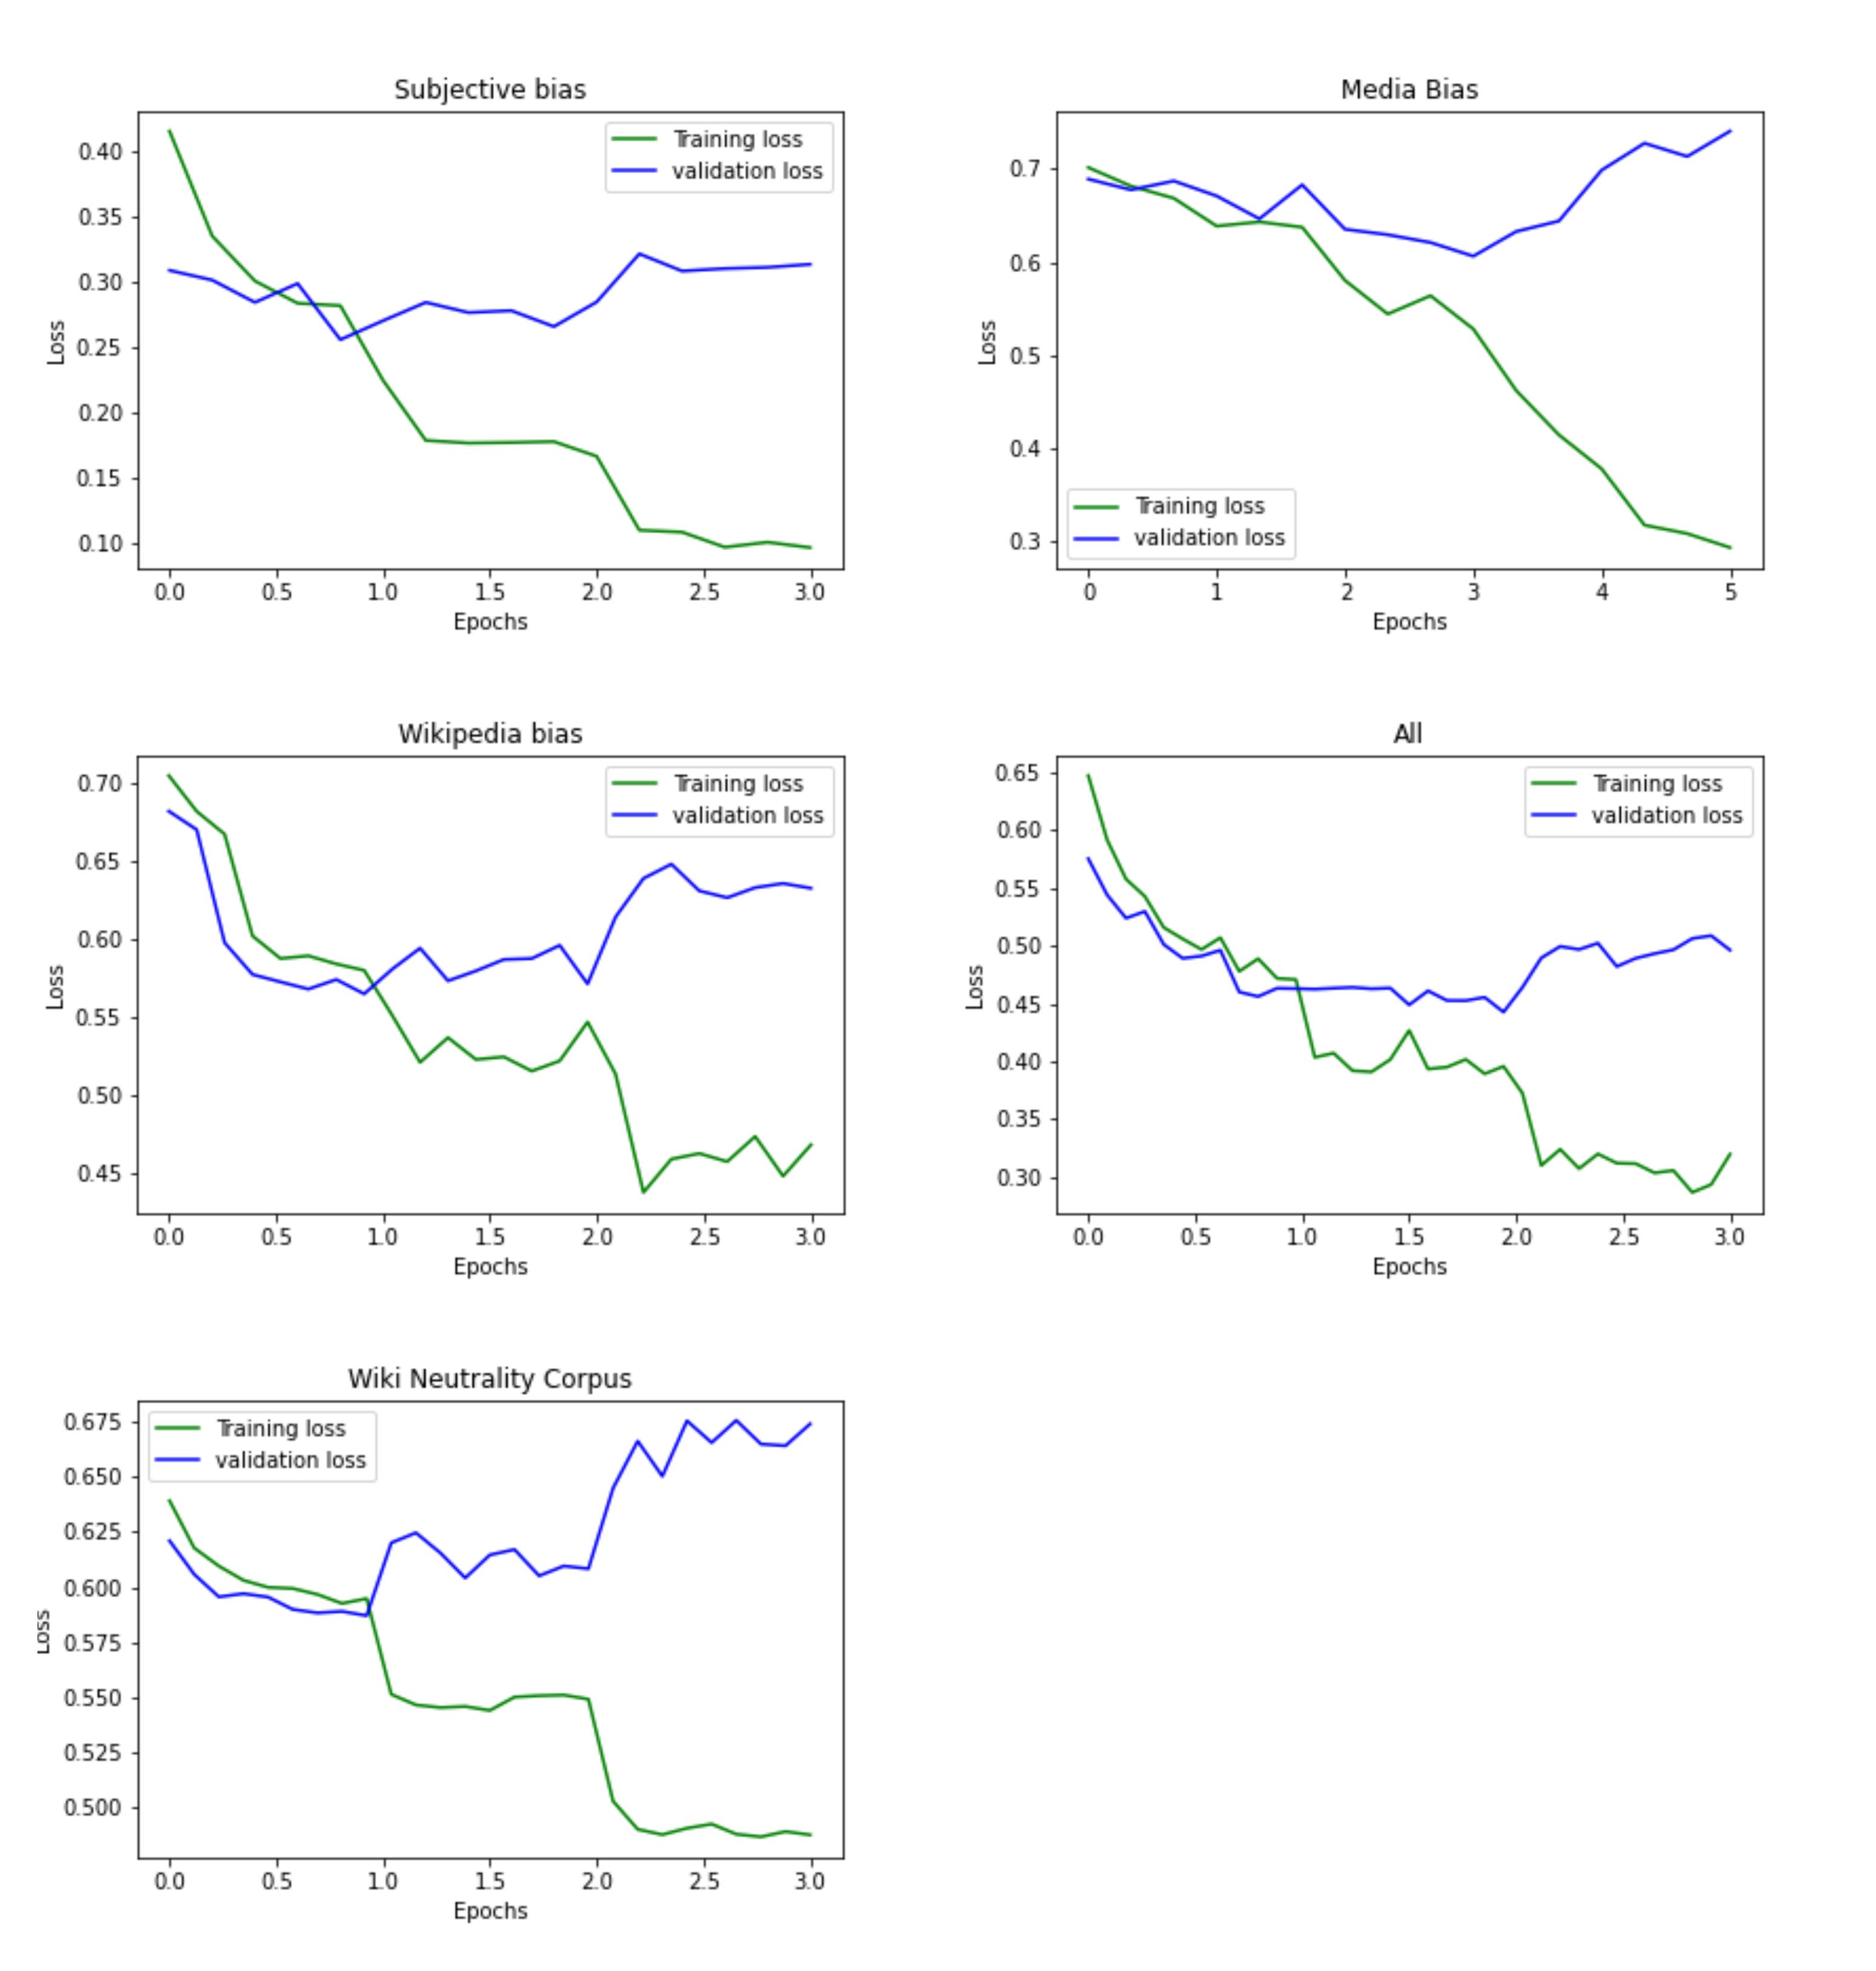
\includegraphics[scale=0.5]{my_modules/multimedia/all_losses.png}
  \caption{Convergence of validation loss over different dataset combinations}
  \label{fig:all_losses}
\end{figure}

Furthermore, I also evaluated pre-trained models on BABE without further fine-tuning, to gain the insight of relatedness to BABE. All results can be seen in \ref{table:4}.

Pre-training on \textbf{ALL} datasets combined resulted in the best performance; however, virtually the same performance was achieved by the model trained on the \textbf{SUBJe} combination. Notably, the SUBJ split represents almost half of all the data (see \ref{fig:cz_data}). Therefore, I assume that the performance of ALL split is high due to the presence of SUBJe.

Pre-training on the other splits hurt the performance. This is mainly because the model had struggled to learn the pre-training tasks in the first place. For example, during pre-training on \textbf{MB}, in the validation set only F1 $\sim40\%$ has been achieved. As opposed to \textbf{SUBJe}, where the model was able to achieve F1 $\sim90\%$ in the first few iterations.


The subjectivity bias as opposed to \gls{mb} is a bit more explicit and more straightforward. Therefore, it can help classify \gls{mb} but not the other way round since the pre-trained SUBJe model achieved only 55\% on BABE. This supports the premise that \gls{mb} is composed of many more superficial linguistic features \ref{features}. However, these results are still greatly influenced by the overall small size and low quality of the datasets.




\section{Results}
The final model for evaluation has been trained with the optimal parameters and pre-trained on all datasets combined. It achieved an F1 score of \textbf{0.804} on a \textbf{test} set. Afterward, for the final model that I share on huggingface, the test set has also been included in the training.


Despite the relatively high performance, the final score in the test set is not representative due to its size. The test set consists of $\sim$ 500 sentences and, therefore, may not adequately represent all bias information. For better evaluation, I propose using a nested cross-validation. However, the computational demand would be very high. 

Possibly, a complete study with more models could be performed, but that would require an enormous number of trained models. Essentially, these results show that there was a minimal gain over the baseline (\textbf{+0.7\%}).

\begin{figure}
\makebox[\textwidth][c]{
  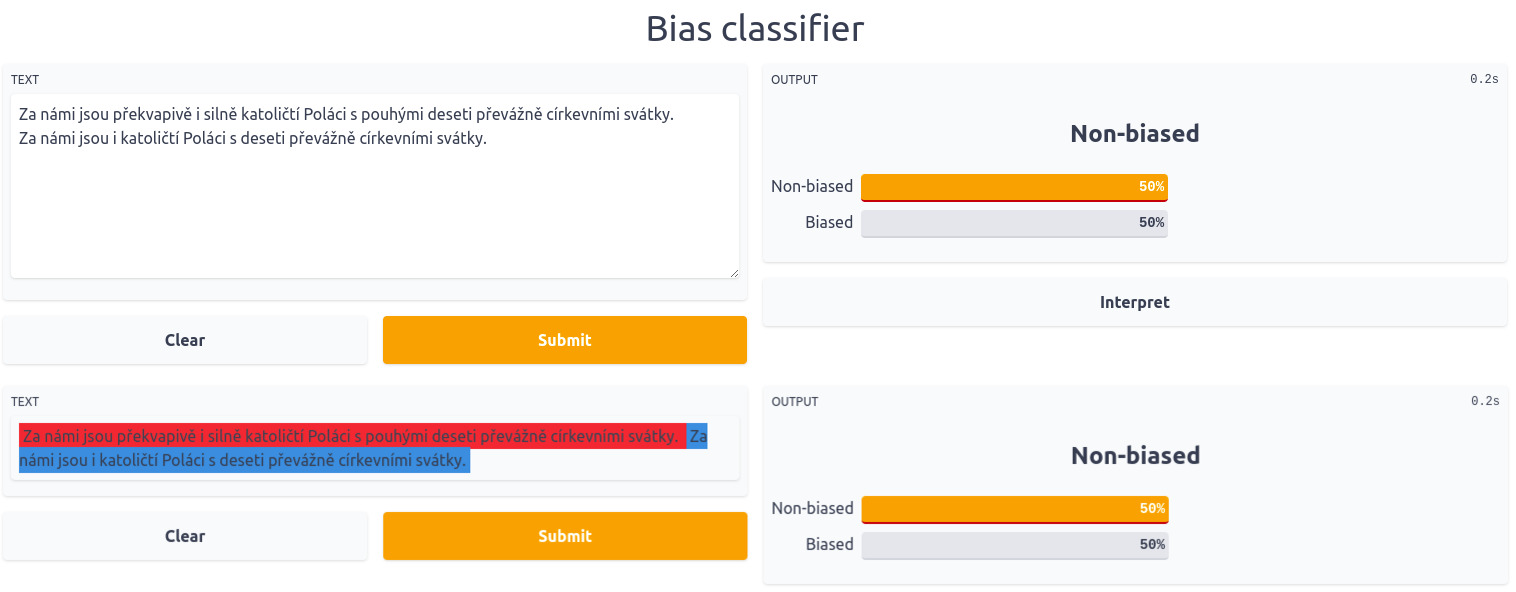
\includegraphics[scale=0.3]{my_modules/multimedia/bias.jpg}
  \caption{Example of the bias classifier demo usage. Red and blue color represent the biased and unbiased annotation respectively.}
  \label{fig:demodemo}
  }
\end{figure}


\subsection{Demo}
Additionally, I provide a simple web demo for the reader to experiment with\footnote{\url{https://huggingface.co/spaces/horychtom/czech_media_bias_detection}}. The use of the demo can be seen in \ref{fig:demodemo}. The backend runs on a \textbf{HuggingFaces spaces} which is a free hosting service for demonstration of \gls{ml} applications. 

The user can insert arbitrary text in Czech language; text is then split into sentences and classified individually. Then the average percentage bias score of the text is displayed. An \textit{interpret} button allows the user to further inspect the classification.


  

\section{Inference on Czech News Samples}\label{inference}

\begin{itemize}
    \item korelovat bias abstraktu (nebo headline) a textu pro jedno medium
    \item vyplotit vyvoj biasu v čase pro jedno medium
    \item vyplotit bias mezi pár mediama
    \item vyplotit bias mezi tématama (bydlení atd)
    \item komentáře jsou skrze "section" ! super
    \item bias není 50\% ! bud je to hodně nebo malo. Bimodal distribution!
    \item use probability of headline bias as a prior
\end{itemize}
